% !TEX root = main.tex
\documentclass[a4paper, UKenglish, 11pt]{uiomaster}
\usepackage{lipsum}
\usepackage[subpreambles=true]{standalone}
\usepackage[table,xcdraw]{xcolor}


% Explain EEG
% Explain how EEG sources can be modeled/simulated (include the first attempt done in 1949)
% Head models (New York Head Model)
% Maybe there should be an implementartion section ?

\begin{document}
\chapter{Results}
As mentioned in chapter 1, an important topic in EEG signal analysis is the inverse problem of going from measured EEG signals to localized equivalent current dipoles, so-called source localization. In this chapter we will present the training and performance of the neural networks presented in chapter 4. Section ... and ... deal with training of the simple feed forward neural network and presenting its results, while section ... will discuss how a convolution neural network can be used to obtain the same results. But first, we will take a look at the dataset being fed to the different networks.

\section{Simulation of EEG Signals}
The cortex matrix of the New York Head Model (NYHM) consists of 74,382 points, representing possible positions for localizing dipole sources. For training the neural networks, we utilize a dataset of self-simulated EEG measurements that correspond to the electromagnetic fields generated by these dipole sources. The dipole sources are randomly positioned within the cortex matrix. To simplify our problem, the amplitude of each dipole is fixed at $10^7$ nA $\mu$m. Additionally,  in the case of single dipole source localization, the direction of the dipole moment is always rotated so that it is normal to the cerebral cortex. In some cases this will result in a dipole moment pointing perpendicular to the skull (directed towards an EEG electorde), while in other cases, due to the structure of the cortex, the dipole moment will point back into the cortex (but eventually towards an EEG electorde). The reason for this is that the human cortex is strongly folded, and the contribution to the EEG signal from a neural population (dipole moment) will depend on whether a dipole is located in a sulcus or a gyrus \cite{naess2021biophysically}. It is important to note that the EEG recordings capture a time series; however, for our analysis, we focus solely on the signal at t = 1, corresponding to the first time step. This allows us to examine the initial snapshot of the EEG signal's spatial distribution and its relationship to the dipole source locations within the cortex.


\subsection{The Effect of dipole location and orientation}
According to Naess et al. (2021) \cite{naess2021biophysically}, EEG signals are not particularly sensitive to small variations in the precise location of neural current dipoles. Despite the common belief that neurons in the upper cortical layers would dominate the EEG due to their proximity to the electrode compared to neurons in deeper layers, such location differences do not significantly affect the EEG signals. This phenomenon can be explained by the fact that the low conductivity of the skull introduces a spatial low-pass filtering effect, which mitigates the impact of location discrepancies.
% Maybe what is meant here is that we therefore only consider the outer corical surface

\begin{figure}[!htb]
    \centering
    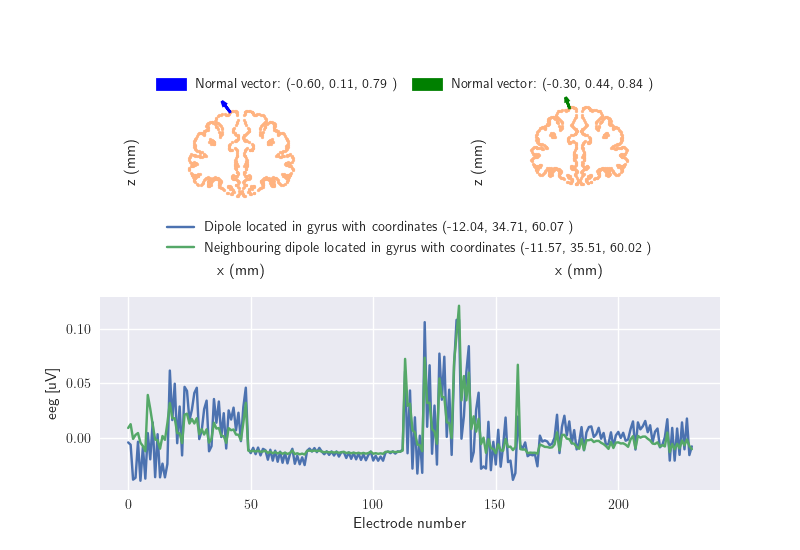
\includegraphics[width=\linewidth]{figures/neighbour_dipoles.png}
    \caption{EEG signal for neighbouring dipoles.}
    \label{fig:neighbour_dipoles}
\end{figure}

However, when considering the orientation of the dipoles relative to the EEG electrodes, the effect becomes noteworthy. To illustrate this, we present in Figure \ref{fig:gyrus_and_sulcus_EEG} the EEG signals obtained from two manually selected dipole locations within the New York head model. These dipoles are situated in a gyrus and a sulcus, respectively, resulting in distinct EEG outcomes. In general, the contribution of an individual current dipole to the EEG signal is maximized when the dipole is located perpendicularly within a gyrus, as depicted in Figure \ref{fig:gyrus_and_sulcus_EEG}B. On the other hand, if a dipole is placed in a sulcus with a perpendicular orientation, a significant EEG contribution can still be observed, but unlike the dipole in the gyrus, it exhibits a more dipolar pattern, as shown in Figure \ref{fig:gyrus_and_sulcus_EEG}C.

\begin{figure}[!htb]
    \centering
    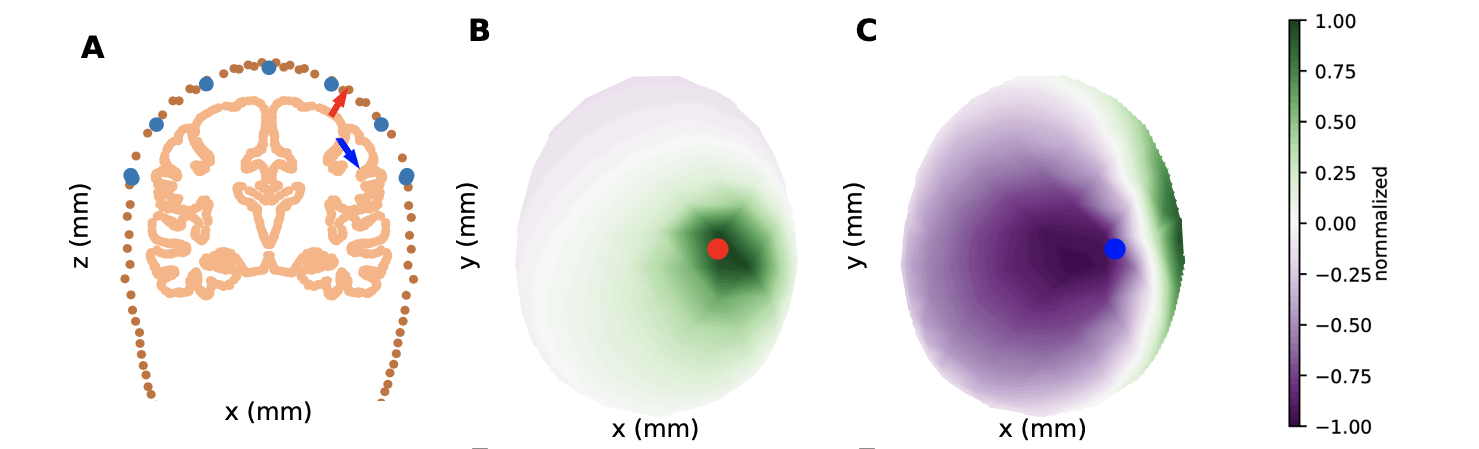
\includegraphics[width=\linewidth]{figures/gyrus_and_sulcus_EEG.png}
    \caption{A: Two selected dipole locations in the New York head model: one in a gyrus (red) and one in a sulcus (blue). The head model is viewed from the side (x, z-plane). Close to the chosen cross-section plane, EEG electrode locations are marked in light blue. Available dipole locations near the cortical cross-section form an outline of the cortical sheet and are marked in pink. The current dipole moment for all cases was $10^7$ nA$\mu$m. B: Interpolated color plot of EEG signal from the gyrus dipole, viewed from the top (x, y-plane). The plotted EEG signal is normalized, with a maximum value of 1.1 $\mu$V. C: Interpolated color plot of EEG signal from the sulcus dipole. The plotted EEG signal is normalized, with a maximum value of 0.7 $\mu$V. \cite{naess2021biophysically}}
    \label{fig:gyrus_and_sulcus_EEG}
\end{figure}

With other words, the EEG outcome is genuinely influenced by the orientation of the current dipole moment generating the signal, as variations in dipole orientation can impact both the direction and distribution of electrical potentials. In Figure \ref{fig:dipole_orientation}, we present the EEG signals obtained from four identical current dipoles with different orientations, situated in distinct hypothetical folding patterns of the cortical surface. Firstly, Figure \ref{fig:dipole_orientation}A and \ref{fig:dipole_orientation}C provide an expanded illustration of the aforementioned scenarios, incorporating additional dipole moments located in a gyrus and a sulcus, respectively. In Figure \ref{fig:dipole_orientation}B, where a collection of dipoles points randomly upwards and downwards, the EEG signal contribution appears to diminish significantly. Conversely, when the dipoles align in the depth direction of the cortex and are distributed across both gyrus and sulcus, we can expect an EEG contribution in between what we saw from Figure \ref{fig:dipole_orientation}A and \ref{fig:dipole_orientation}B, as depicted in Figure \ref{fig:dipole_orientation}D. Lastly, Figure \ref{fig:dipole_orientation}E demonstrates the minimal EEG contribution observed when the dipoles are divided between two opposing sulci.


\begin{figure}[!htb]
    \centering
    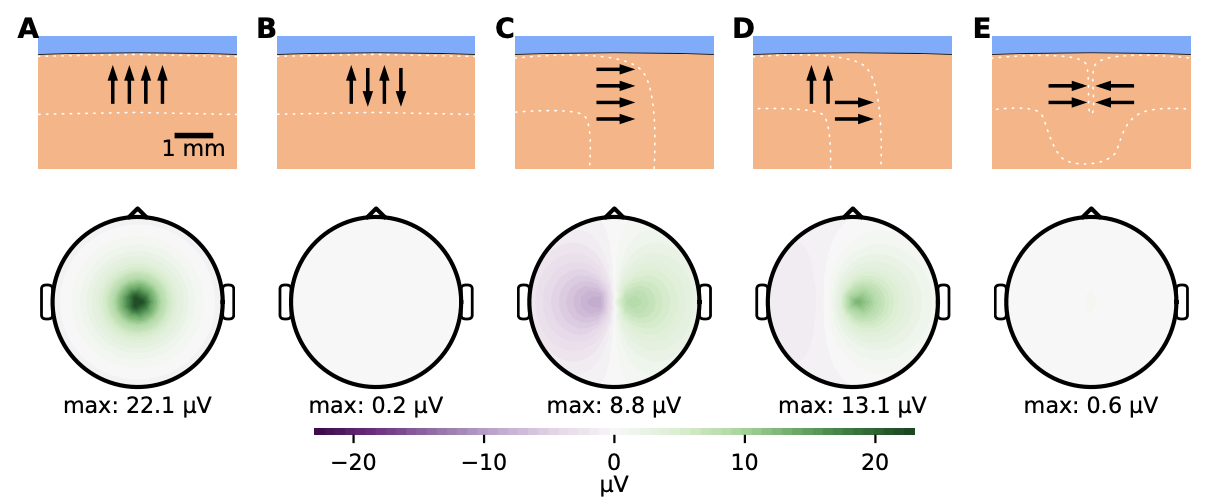
\includegraphics[width=\linewidth]{figures/dipole_orientation.png}
    \caption{Different folding patterns of the cortical surface are represented by white dashed lines. EEG signals are calculated from four identical current dipoles with varying orientations. A: Dipoles aligned in the same direction within a gyrus. B: Dipoles pointing in opposite directions within a gyrus. C: Dipoles aligned in the same direction within a sulcus. D: Dipoles distributed between a gyrus and a sulcus, pointing towards the cortical surface. E: Dipoles divided between opposing sulci, pointing towards the cortical surface.
    All panels have a dipole moment magnitude of 10 nAm, and the dipoles are positioned at the centers of the arrows in the top row.}
    \label{fig:dipole_orientation}
\end{figure}

% This is not the case for a simple dipole moment, but might be an issue when giving the populations a radii
% In our analysis, we simplify the scenario by considering one current dipole at a time, which allows us to avoid cancellations of potentials and obtain simpler EEG potentials. While this simplification may not capture the full complexity of neural activity, it provides us with a clearer understanding of the relationship between dipole orientation and EEG signals.


\subsection{Noise}
% As for all experimental data, real EEG recordings contain noise. Artifacts are signals recorded by EEG but with a origin different from those generated by human brain activity. As some artifact may mimic true epileptiform abnormalities or seizures, awereness of artifacts and methods for distinguishing such signals from brain waves is highly important \cite{sazgar2019eeg}.
%
% There are two different dypes of artifacts, classified according to their origin. Physiological artifacts originate from the patient itself, where the most usual ones are ocular activity, muscle activity, cardiac activity, perspiration and respiration. Technical artifacts, on the other hand, is generated from the environment of the patient, such as cable and body movements or electromagnetic interferences \cite{bitbrain}.
%
% Filtering techniques are usually utilized in order to remove artifact from EEG before analyzation of the recordings. But, when it comes to the simulated EEG data of ours, we are in no need to remove such noise, as there simply is none. The simulated EEG data can be understood as already filtered data that has undergone preprocessing steps, to ensure a high signal-to-noise ratio \cite{wiki-snr}. Moreover we understand the simulated data as an averaged measure of the typical EEG time series, meaning that our final data only consist of one dimension, or one time step. However, in order to avoid overfiting and for other tecnical detailes, we do need to add noise to the data before feeding it to the neural network. Therefore, to the final dataset of ours we add normally distributed noise of 10 $\%$, with mean 0. The standard deviation of the noise is calculated from the simulated eeg result, and lays around 1.


Experimental EEG recordings inevitably contain noise, which can interfere with the accurate analysis of brain activity. Artifacts, which are signals recorded by EEG but originating from sources other than the human brain, pose a particular challenge. Some artifacts can mimic genuine epileptiform abnormalities or seizures, underscoring the importance of identifying and distinguishing them from true brain waves \cite{sazgar2019eeg}.

Artifacts can be classified into two categories based on their origin. Physiological artifacts arise from the patient's own physiological processes, including ocular activity, muscle activity, cardiac activity, perspiration, and respiration. Technical artifacts, on the other hand, originate from external factors such as cable and body movements or electromagnetic interferences \cite{bitbrain}.

Filtering techniques are commonly employed to remove artifacts from EEG recordings prior to analysis. However, in the case of simulated EEG data, the need for artifact removal is eliminated as the data inherently lacks noise. Simulated EEG data can be considered as pre-filtered and preprocessed, ensuring a high signal-to-noise ratio (SNR) \cite{wiki-snr}. Nevertheless, to avoid overfitting and account for technical considerations, it is necessary to introduce noise to the data before feeding it into the neural network. This introduction of the noise is vital in order to make the trained neural network more likely to accurately handle real EEG recordings.

In our approach, we recognize that the introduction of noise to the simulated EEG data is an essential step to enhance the robustness of the trained neural network and ensure its ability to handle real EEG recordings effectively. Although the specific characteristics and quantity of noise have not been the primary focus of our study, we have opted for a straightforward approach. Our final dataset incorporates normally distributed noise with a mean of 0 and a standard deviation equal to 10$\%$ of the standard deviation observed in the simulated EEG recordings. By introducing this noise, we introduce random variations around each data point while preserving the overall normalization properties of the dataset.

\begin{figure}[!htb]
    \centering
    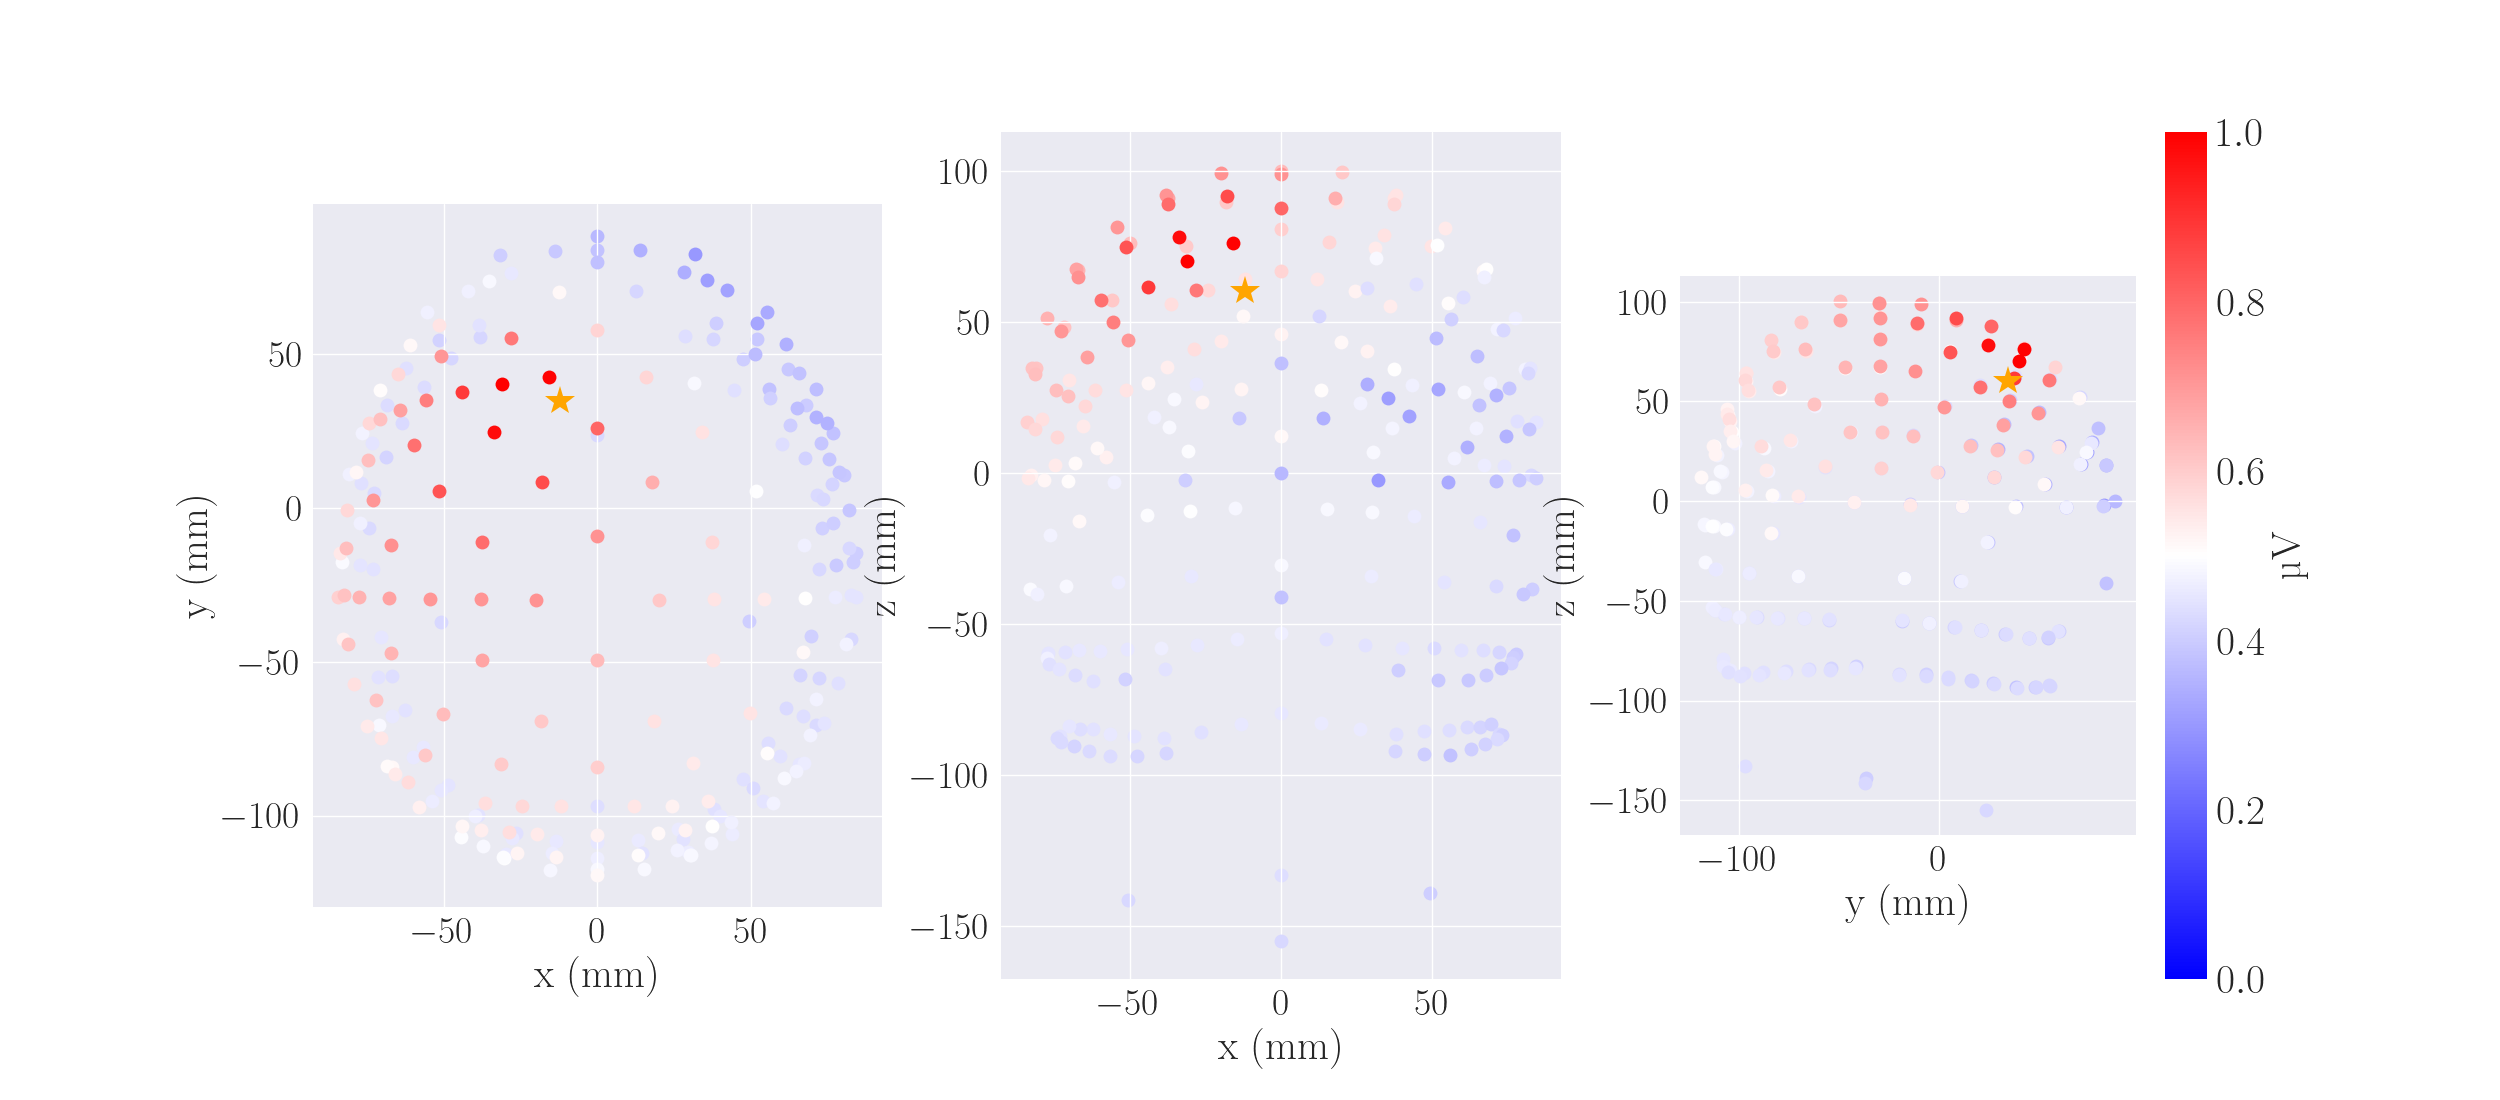
\includegraphics[width=\linewidth]{figures/simple_dipole_eeg_field_noise_10.png}
    \caption{EEG for a sample containing one single current dipole source at a random position within the celebral cortex. As for all samples, 10 percent of normally distributed noise has been added to the original signal. The EEG measure is seen from both sides (x-, z-plane and y-, z-plane) and above (the x-, y-plane). EEG electrode locations are presented as filled circels, where the color of the fill represents the amplitude of the measured signal for the given electrode. The position of the current dipole moment is marked with a yellow star.}
    \label{fig:eeg_field_1_dipole_example}
\end{figure}

\subsection{The dataset}
The training dataset for a simple feed-forward neural network comprises 50,000 rows, where each row corresponds to a single sample or patient. Within the dataset, there are 231 columns representing the features, which denote the EEG measurements recorded at each electrode. Consequently, the design matrix has a size of 50,000 x 231.

Figure \ref{fig:eeg_field_1_dipole_example} presents an example of the input EEG data for a single sample, with 10$\%$ noise added. The illustration showcases the EEG results obtained from a sample containing a solitary current dipole source positioned randomly within the cerebral cortex. The dipolar pattern in the figure indicates that the dipole is located within a sulcus. The EEG measure is visualized from multiple perspectives, including the x-z plane, y-z plane, and the x-y plane. The electrode locations are represented by filled circles, with the color of the fill indicating the amplitude of the measured signal at each electrode. The position of the current dipole moment is denoted by a yellow star. As observed from the figure, the EEG signal for this specific sample ranges from -1 to 1 μV.


\section{Localizing Single Dipole Sources}

% One example on coordinate prediction

% include the neural net that has been used

The first problem we want to introduce for our neural network, DiLoc, is simply the standard inverse problem. By feeding the network EEG data corresponding to the electrical activity from dipoles distributed randomly in the cerebral cortex for different samples, we want the network to output the x-, y- and z-coordinates of the localization of the current dipoles. In figure \ref{fig:single_dipole_accuracy} we have provided the loss of our network as a function of training epochs. It is apparent that the the network picks up on the patterns of the data, as we clearly can observe the trend of decreasing loss with an increasing number of epochs. Moreover, we can see that the both training and validation loss stabilizes at around 400 epochs.

\begin{figure}[!htb]
    \centering
    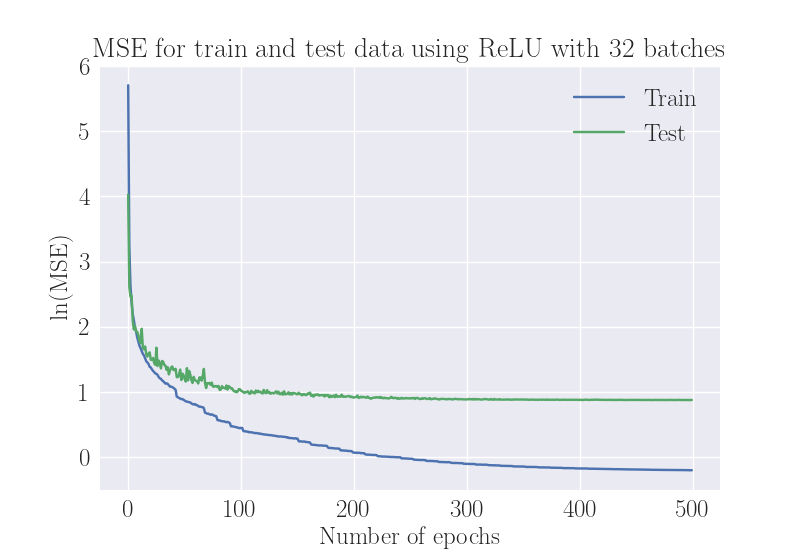
\includegraphics[width=\linewidth]{figures/MSE_simple_dipole_lr0.001_RELU_500_50000_ReLU_32_500_N_dipoles_1.png}
    \caption{The loss for the simple Feed Forward Neural Network with 50 000 samples and ReLU as activation function. }
    \label{fig:single_dipole_accuracy}
\end{figure}

In Table \ref{table:error_simple_dipole} we have provided the performance of the network by concidering different error metrics. The mean absolute error (MAE) values for the x-, y-, and z- coordinates rnage from 0.8300 mm to 0.8998 mm. This means that, on average, the network's predictions have an error smaller than 1 mm in each coordinate. Considering the range of the coordinates, the MAE values represent a reasonable level of accuracy. The mean squared error penalizes larger errors/outliers more severely than MAE since it involves squaring the differences. In our case the MSE values for the different coordinates range from 1.2134 mm to 1.4110 mm. The hugher MSE values suggest that the predictions of the network may have larger errors in some cases, resulting in a higher average squared difference. However, the magnitude of the mean squared errors is still whithin a reasonable range when analyzing them in the context of the coordinates ranges. Finally the root mean squared error provides a measure of the standard deviation of the errors and helps to understand the spread of errors around the mean. The RMSE values of ours are slighly lower than the corresponding MSE values with a range from 1.1016 mm to 1.1878 mm. The table also presents the error metrics calculated for the euclidean distance. For both MAE, MSE and RMSE the value is higher than the individual coordinate errors, indicating that the errors in the x, y, and z coordinates are not perfectly aligned and contribute to the overall distance. It is worth mentioning that specific points in the cortex matrix may potentially contribute more to the errors. Further investigation could be performed to identify any specific patterns or regions in the cortex that exhibit higher error rates. However, overall the results indicate that the network is able to predict the dipole location with reasonable accuracy. While there are some errors in the predictions, the errors are generally within an acceptable range.

% Please add the following required packages to your document preamble:
% \usepackage[table,xcdraw]{xcolor}
% If you use beamer only pass "xcolor=table" option, i.e. \documentclass[xcolor=table]{beamer}
\begin{table}[!htb]
\begin{tabular}{l|cccc|}
\cline{2-5}
\rowcolor[HTML]{CBCEFB}
\cellcolor[HTML]{FFFFFF}                           & \multicolumn{4}{c|}{\cellcolor[HTML]{CBCEFB}{\color[HTML]{000000} \textbf{Error for different target values}}}                                                                                                                                                                                                                                                                                                                                                     \\ \cline{2-5}
\rowcolor[HTML]{EFEFEF}
\cellcolor[HTML]{FFFFFF}\textbf{}                  & \multicolumn{1}{l|}{\cellcolor[HTML]{EFEFEF}\begin{tabular}[c]{@{}l@{}}x-coordinate\\ {[}mm{]}\end{tabular}} & \multicolumn{1}{l|}{\cellcolor[HTML]{EFEFEF}\begin{tabular}[c]{@{}l@{}}y-coordinate \\ {[}mm{]}\end{tabular}} & \multicolumn{1}{l|}{\cellcolor[HTML]{EFEFEF}\begin{tabular}[c]{@{}l@{}}z-coordinate \\ {[}mm{]}\end{tabular}} & \multicolumn{1}{l|}{\cellcolor[HTML]{EFEFEF}\begin{tabular}[c]{@{}l@{}}Euclidean \\ Distance {[}mm{]}\end{tabular}} \\ \hline
\multicolumn{1}{|l|}{\cellcolor[HTML]{EFEFEF}MAE}  & \multicolumn{1}{c|}{0.8300}                                                                                  & \multicolumn{1}{c|}{0.8998}                                                                                   & \multicolumn{1}{c|}{0.8419}                                                                                   & 0.8573                                                                                                              \\ \hline
\multicolumn{1}{|l|}{\cellcolor[HTML]{EFEFEF}MSE}  & \multicolumn{1}{c|}{1.2638}                                                                                  & \multicolumn{1}{c|}{1.4110}                                                                                   & \multicolumn{1}{c|}{1.2134}                                                                                   & 1.2961                                                                                                              \\ \hline
\multicolumn{1}{|l|}{\cellcolor[HTML]{EFEFEF}RMSE} & \multicolumn{1}{c|}{1.1242}                                                                                  & \multicolumn{1}{c|}{1.1878}                                                                                   & \multicolumn{1}{c|}{1.1016}                                                                                   & 1.1385                                                                                                              \\ \hline
\end{tabular}
\caption{\textbf{Evaluation of the network performance utializing different Error Metrics.} \newline
Network performance on test dataset consisting of 1000 samples. The errors are measured using Mean Squared Error (MSE), Mean Absolute Error (MAE), and Root Mean Squared Error (RMSE).}
\label{table:error_simple_dipole}
\end{table}

% You can include a little bit more here. Find some examples in the figure coordinate system. Give average error in the crossection.
In order to conduct a detailed analysis of the network's performance, Figure \ref{fig:MAE_crossections} presents the Mean Absolute Error (MAE) for various dipole locations within the New York head model cortex matrix. The figure provides valuable insights into the distribution of errors across different regions of the cortex, with three cross-sections—front, top, and side—depicted for examination.

The MAE values presented in the panels are consistently below 1 mm, which indicates a high level of accuracy in the network's predictions. These results are promising and demonstrate the network's ability to estimate dipole locations with a high level of precision. The panels also offer an opportunity to assess whether the network performs differently for dipoles located in the gyrus compared to the sulcus.

Initially, it might be assumed that EEG signals originating from dipoles in the sulcus present greater challenges for the network's analysis and prediction. This assumption is based on the deeper placement of dipoles within the sulcus compared to those in the gyrus, as well as the potential complexities introduced by the dipole's orientation within the cortex. However, upon closer examination of Figure \ref{fig:MAE_crossections}, it becomes evident that the distribution of MAE values does not exhibit a clear correlation with the brain's structural characteristics. The MAE values appear to vary randomly across different regions, indicating that the network's performance is not significantly influenced by the distinction between the gyrus and sulcus.


Surprisingly, the Mean Absolute Error (MAE) for dipoles located in the sulcus is 1.1075 mm, which is even smaller than the MAE for dipoles in the gyrus measuring 1.2458 mm. This finding directly contradicts the initial assumption and suggests that the network exhibits great precision in predicting dipole locations regardless of their placement within the cortex. The lower MAE values specifically for dipoles in the sulcus  the network's remarkable ability to effectively capture the complex features and variations associated with deeper cortical placements. Moreover, the results highlight the network's robustness and accuracy across different cortical structures, reinforcing its potential for accurate dipole localization within the human brain.


\begin{figure}[!htb]
    \centering
    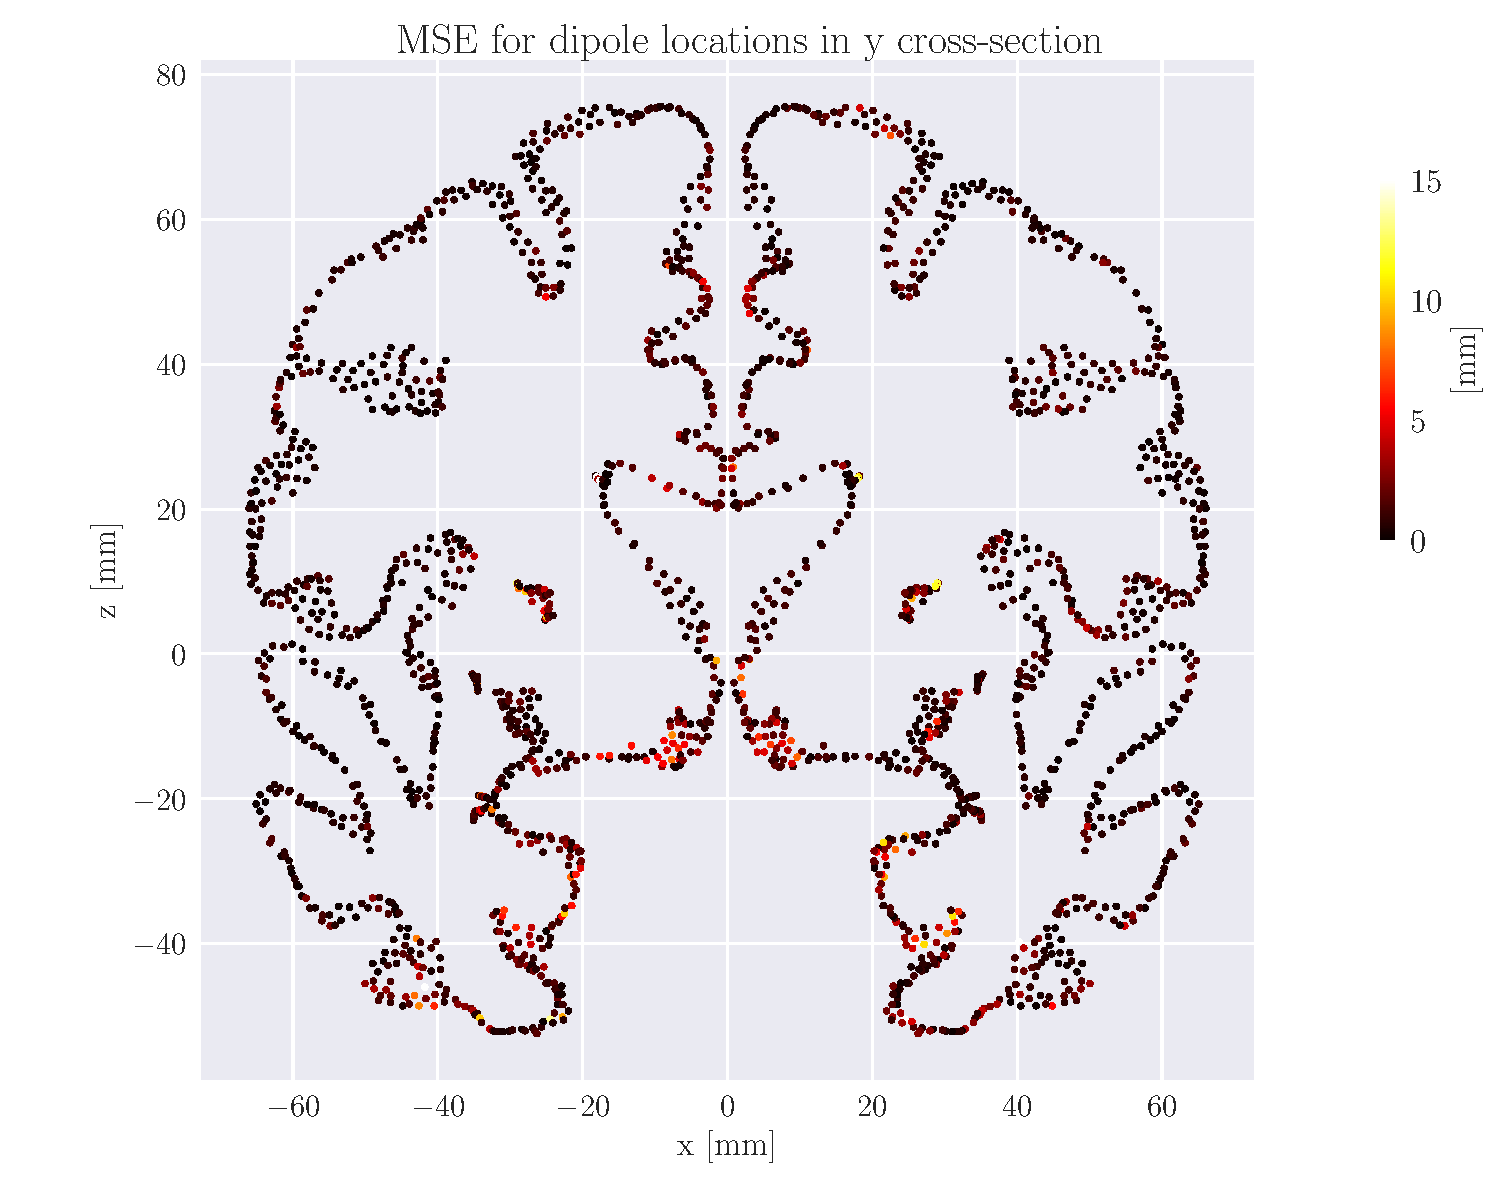
\includegraphics[width=0.7\linewidth]{figures/NEW_simple_dipole_error_Euclidean Distance_0.pdf}
    \vspace{10pt} % Adjust the vertical spacing between the images
    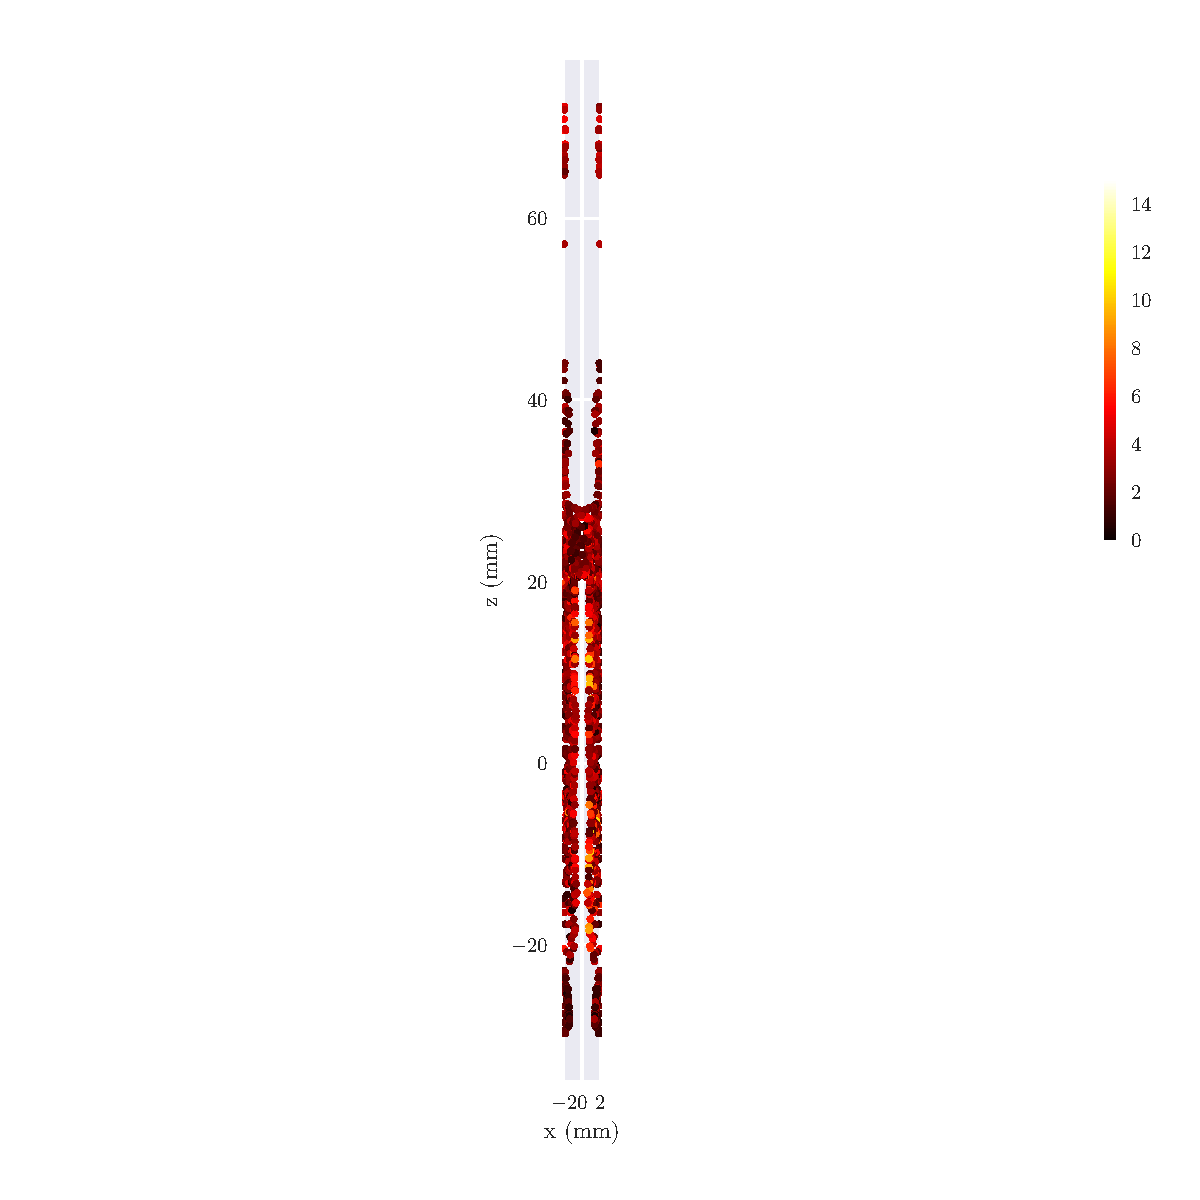
\includegraphics[width=0.7\linewidth]{figures/NEW_simple_dipole_error_Euclidean Distance_1.pdf}
    \vspace{10pt} % Adjust the vertical spacing between the images
    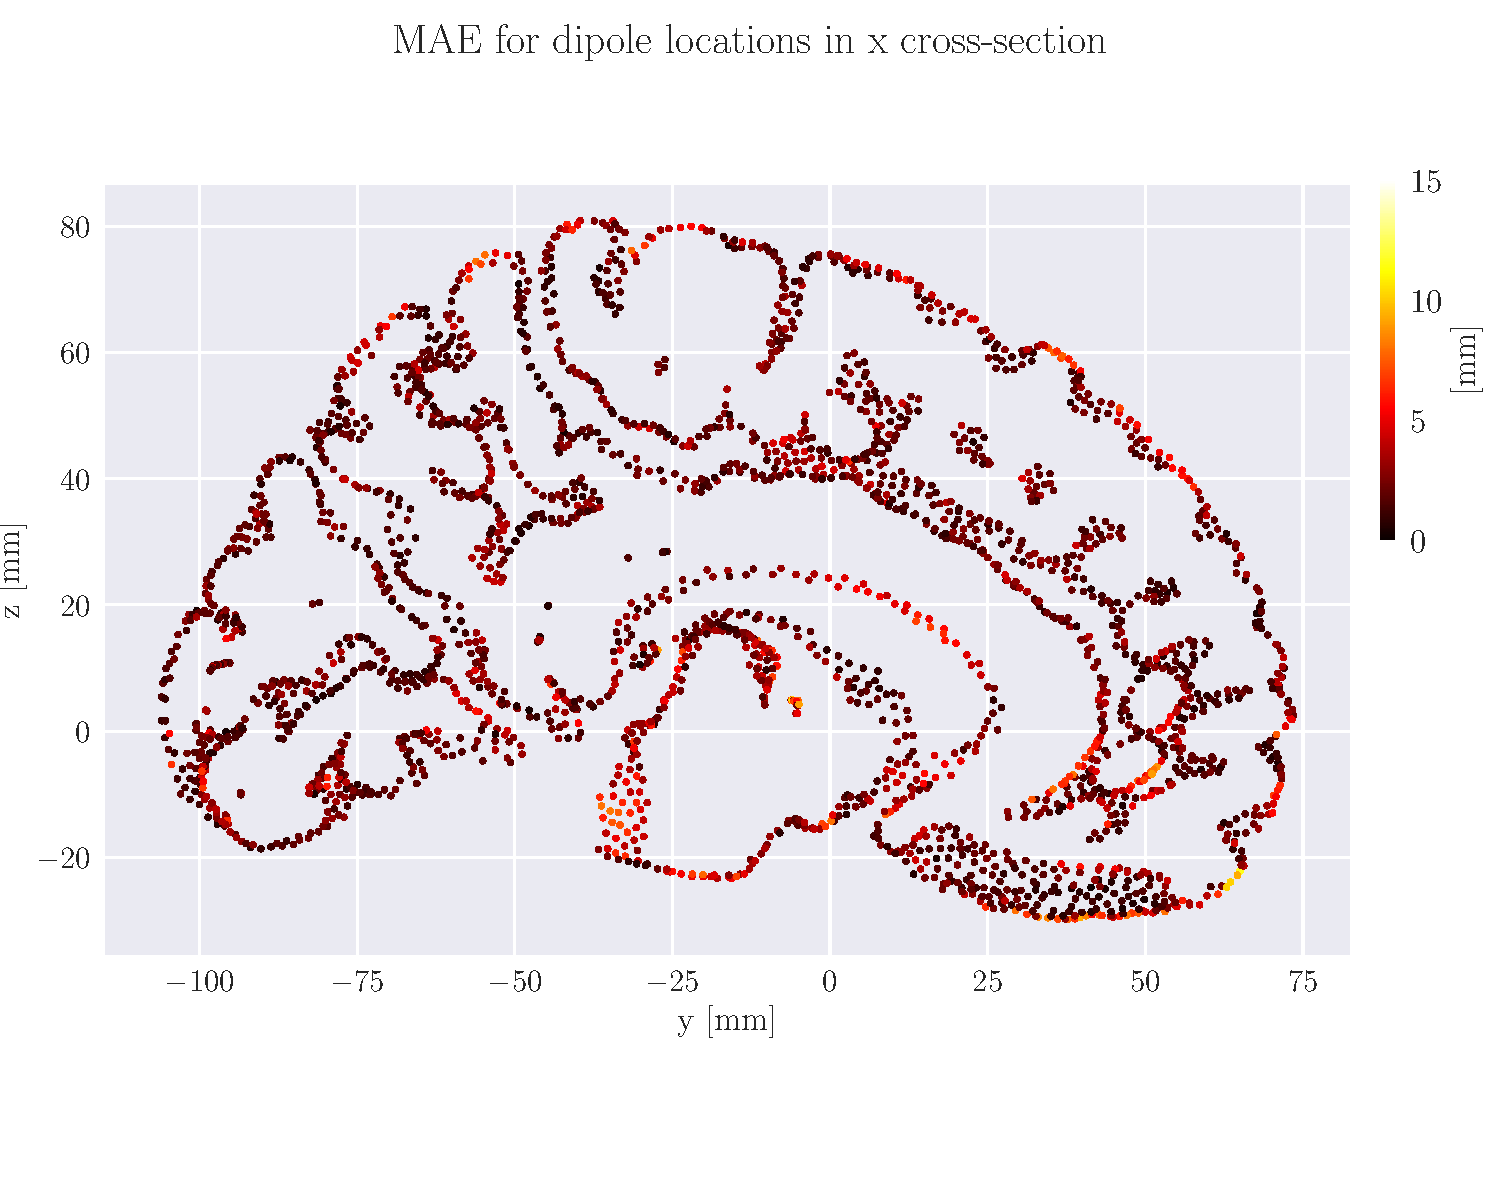
\includegraphics[width=0.7\linewidth]{figures/NEW_simple_dipole_error_Euclidean Distance_2.pdf}
    \caption{Different cross-sections of the cortex from the New York head model, seen from front, top and side. Each point represents a possible position in the cortex matrix. The color of the each point indicates the mean absolute error (MAE) of the neural network when predicting that specific dipole location.}
    \label{fig:MAE_crossections}
\end{figure}



\section{Convolution Neural Network Approach for localizing single dipole sources}

Some results for the prediction of location for single current dipoles.


\begin{figure}[!htb]
\centering
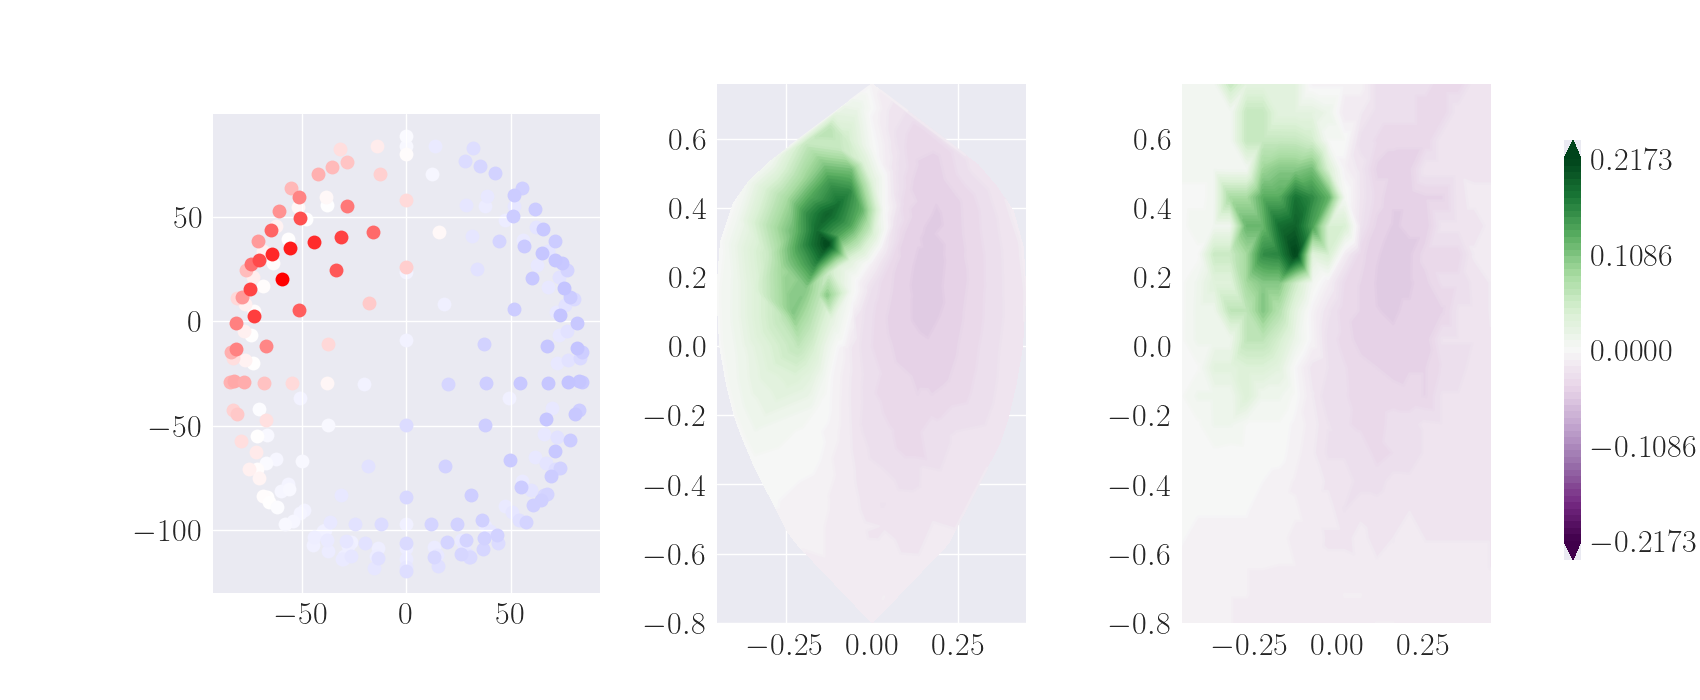
\includegraphics[width=\linewidth]{../Code/plots/finals/new_eeg_dipole_pos_0.png}
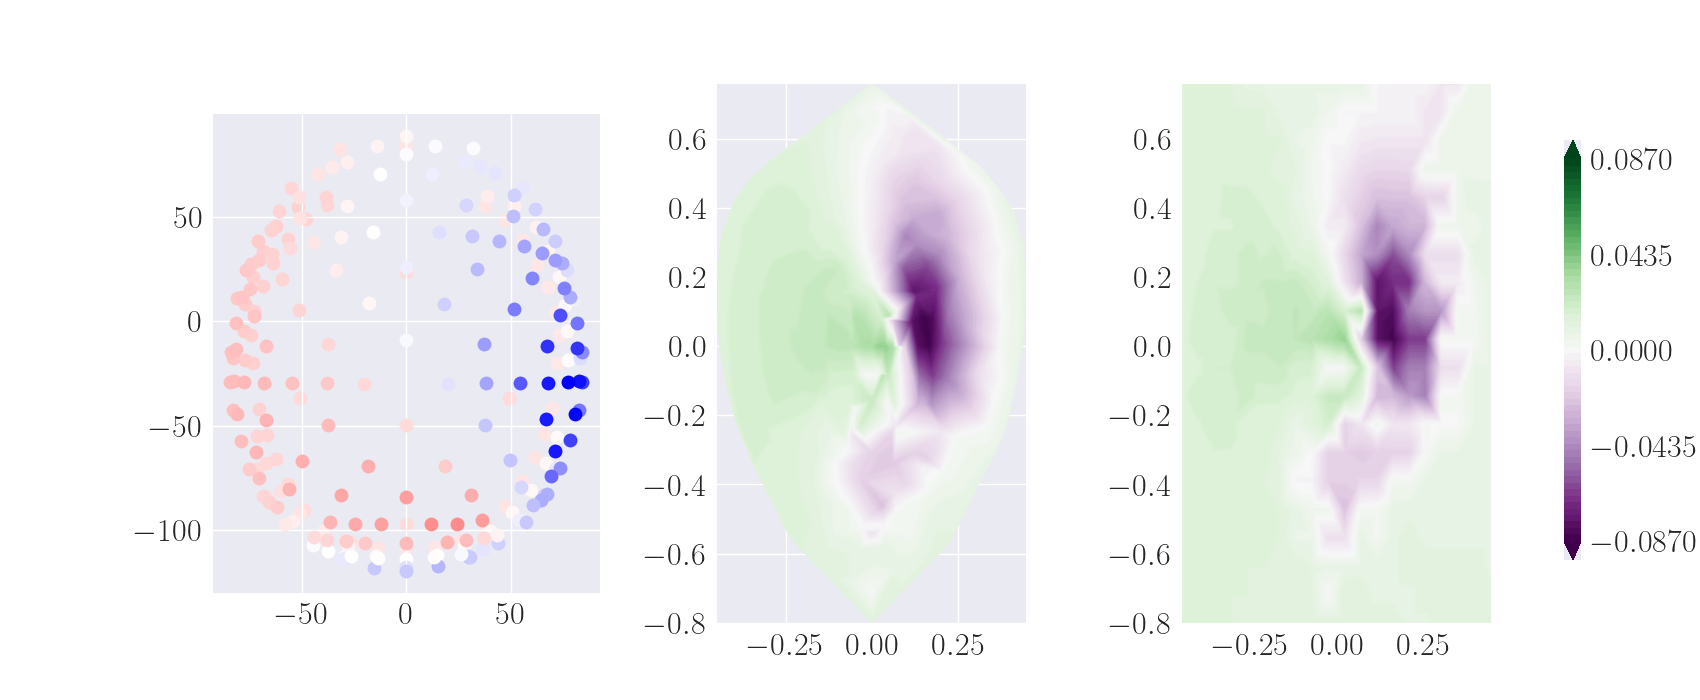
\includegraphics[width=\linewidth]{../Code/plots/finals/new_eeg_dipole_pos_4.png}
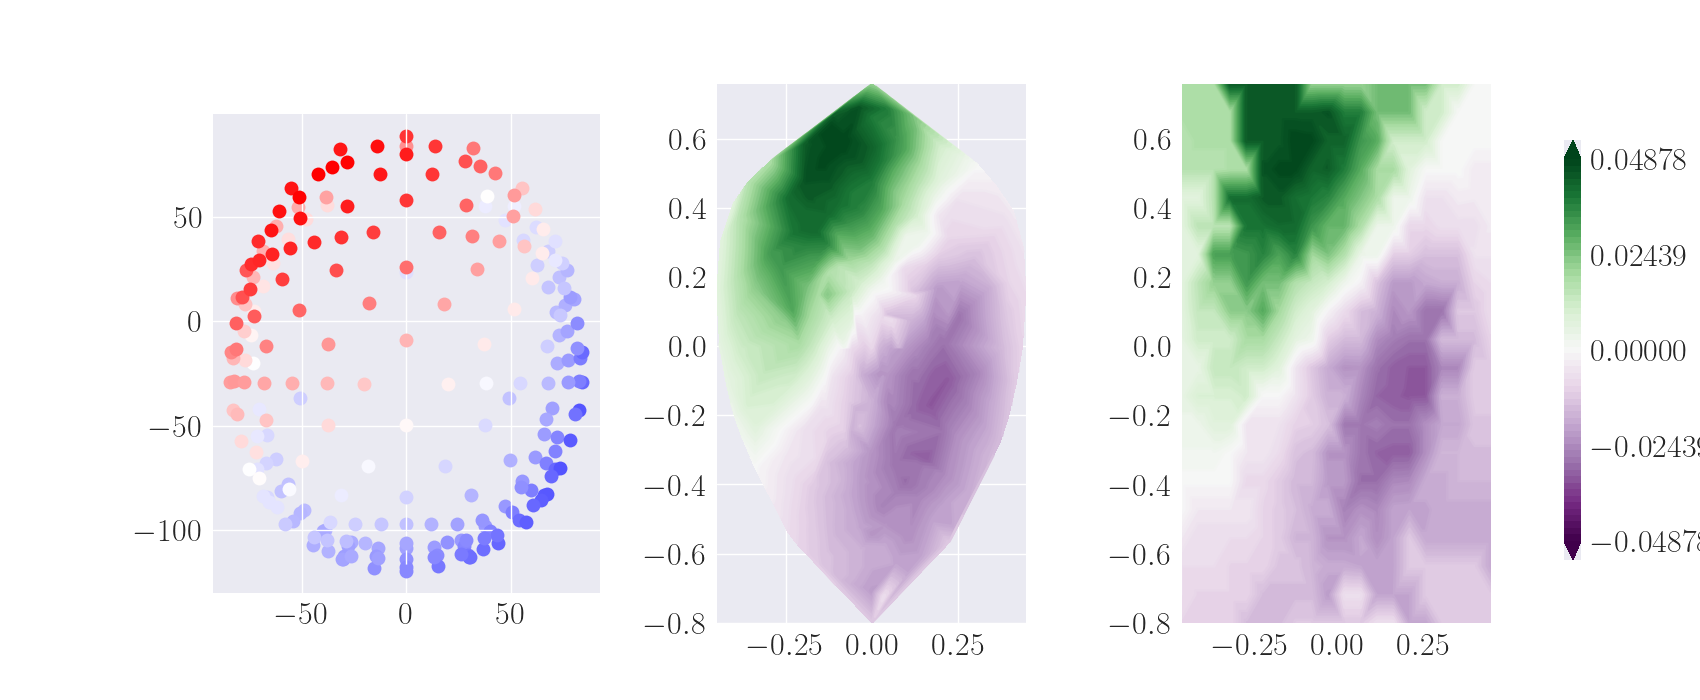
\includegraphics[width=\linewidth]{../Code/plots/finals/new_eeg_dipole_pos_6.png}

\caption{\newline
\textbf{Right}: EEG measure for 3 different samples measured in $\mu V$. \newline
\textbf{Middle and Left}: Illustration of the interpolation of the EEG data into two-dimensional matrix.}
\label{fig:eeg_dipole_pos_0}

\end{figure}

\begin{figure}[!htb]
    \centering
    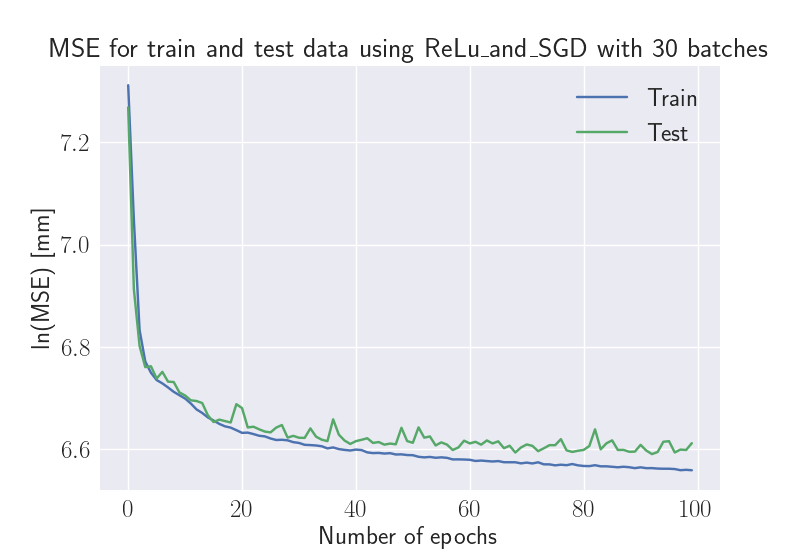
\includegraphics[width=\linewidth]{../Code/plots/finals/MSE_CNN_dipoles_2_interpolated_CNN_20x20_10000_ReLu_and_SGD_30_100.png}
    \caption{The validation accuracy for Convolutional Neural Network with 10 000 samples (20x20 matrix) with ReLU activation function. }
    \label{fig:single_dipole_accuracy_CNN_2d}
\end{figure}

% \begin{figure}[!htb]
%     \centering
%     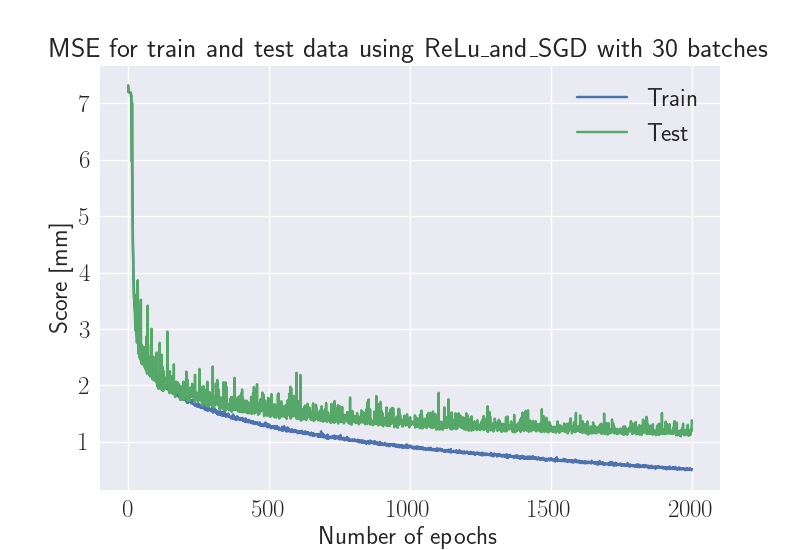
\includegraphics[width=\linewidth]{../Code/plots/CNN/MSE_interpolated_CNN_20x20_10000_ReLu_and_SGD_30_2000.png}
%     \caption{The validation accuracy for Convolutional Neural Network with 10 000 samples (20x20 interpolated matrix) with ReLU activation function. }
%     \label{fig:single_dipole_accuracy_CNN}
% \end{figure}


\end{document}